\newcommand{\Cdel}{\ensuremath{c_{del}}}
\newcommand{\Cins}{\ensuremath{c_{ins}}}
\newcommand{\Cupd}{\ensuremath{c_{upd}}}

\newcommand{\AfullDecomposition}{\ensuremath{\mathcal{A}}}
\newcommand{\FrelevantSubforests}{\ensuremath{\mathcal{F}}}
\newcommand{\pluseq}{\stackrel{+}{=}}
\newcommand{\AlgCase}{$\left\{\rule{0pt}{\baselineskip}\right.$\parbox{\textwidth}}

\newcommand{\rtedCostSum}[3]{\sum_{{#1}' \in #1 - \gamma^{#2}(#1)}cena({#1}', #3)}
\newcommand{\set}[1]{\ensuremath{\{#1\}}}


%indentation in code:
\algdef{SE}[SUBALG]{Indent}{EndIndent}{}{\algorithmicend\ }
\algtext*{Indent}
\algtext*{EndIndent}




\chapter{Mapovanie medzi RNA stromami}

Ako sme spomínali v predchádzajúcich častiach, biológovia očakávajú, že
podobné RNA molekuly (pozeráme na sekundárnu štruktúru) budú mať aj podobnú vizualizáciu.
To znamená, že nakreslenia sa majú líšiť iba v~rozdielnych častiach.

Vieme už, že RNA a~jej sekundárnu štruktúru vieme reprezentovať ako usporiadaný strom.
Táto kapitola nám dá návod, ako nájsť najmenší počet úprav, ktorý prevedie jeden strom
na iný. Vďaka tomu, že poznáme vizualizáciu jednej molekuly - vieme rozvrhnutie jej báz na
obrázku a~dokážeme ju previesť na cieľovú molekulu, rovnaké štruktúry budú rovnako vizualizované.

To nás privádza k~algoritmu \textit{tree-edit-distance, TED}. Je obdobou Levenshteinového
string-edit-distance algoritmu (\citet{LEVENSHTEIN}).
Ten počíta editačnú vzdialenosť medzi dvomi reťazcami a~transformuje
jeden reťazec na druhý.

Problém u~reťazcov je špeciálnym prípadom TEDu, kedy nám stromy zdegenerovali
na cesty (spojový zoznam).





\section{Tree-edit-distance algoritmus}

Základ TED algoritmu je v~rekurzivnom vzorci \ref{eq:ted}. Vzdialenosť medzi
stromami \tree{F} a~\tree{G}, $\delta(F, G)$ je definovana ako minimálny počet editačných operácií,
ktoré z~\tree{F} urobia \tree{G}. Používame štandardne editačné operácie - delete, insert, update.

\begin{figure}[H]
\centering
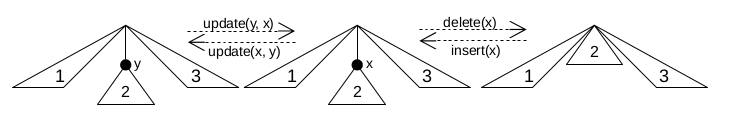
\includegraphics[width=140mm, height=30mm]{../img/TED_operations.png}
\caption{Ukážky TED operácií}
\label{obr:TED_operations}
\end{figure}

Delete, operácia zmazania vrcholu, znamená pripojiť k jeho predkovi všetkých jeho
potomkov so zachovaním poradia medzi nimi. Insert, vkladanie vrcholu, je opačná
operácia. Vkladáme vrchol medzi predka a~nejakých jeho, po sebe nasledujúcich
potomkov. Update iba zmení hodnotu vo vrchole stromu.
Tieto operácie sú názorne ukázané na obrázku \ref{obr:TED_operations}.

\begin{definice}[Editačná vzdialenosť]
  Nech \tree{F} a~\tree{G} sú dva stromy. Editačna vzdialenosť (tree-edit-distance, $\delta(F, G)$),
  medzi \tree{F} a~\tree{G} je rovná minimálnej cene, za ktorú strom F transformujeme na G.
\end{definice}

Rekurzia \ref{eq:ted} počíta vzdialenosť medzi dvoma lesmi \tree{F} a \tree{G}.
\Cdel, \Cins a~\Cupd sú ceny zmazania, vloženia a~updatu vrcholu v~strome
a~$r_{F}$ a~$r_{G}$ sú korene \tree{F}, respektíve \tree{G} a~to buď obidva najpravejšie
alebo najľavejšie (tzn. vyberieme najpravejší/najľavejší strom lesa a~jeho koreň).


\begin{figure}
  \begin{subequations}
  \begin{align*}
    \begin{split}
    \delta(\emptyset, \emptyset) &=
      0
      \\
    \delta(F, \emptyset) &=
      \delta(F - r_{F}, \emptyset) + \Cdel(r_{F})
      \\
    \delta(\emptyset, G) &=
      \delta(\emptyset, G - r_{G}) + \Cins(r_{G})
    \end{split}
    \\[1ex]
    \delta(F, G) &=
      \begin{cases}
        \delta(F - r_{F}, G) + \Cdel(r_{F}) \\
        \delta(F, G - r_{G}) + \Cins(r_{G}) \\
        \delta(F - F_{r_{F}}, G - G_{r_{G}}) \\
          \quad \quad + \delta(F_{r_{F}} - r_{F}, G_{r_{G}} - r_{G}) \\
          \quad \quad + \Cupd(r_{F}, r_{G})
      \end{cases}
  \end{align*}
  \end{subequations}
  \caption{Rekurzívny vzorec pre výpočet tree-edit-distance od \citet{DMRW} a \citet{RTED}}
  \label{eq:ted}
\end{figure}






\section{\sloppy Vývoj algoritmu - rekurzia a~dynamické programovanie}

Algoritmus TED prešiel vývojom postupne od \citet{TAI}, ktorý predstavil algoritmus
na výpočet editačnej vzdialenosti s~priestorovou a~časovou zložitosťou
\O{$m^3 \cdot n^3$}. Algoritmus vylepšili \citet{ZHANGSHASHA} vypozorovaním toho,
že nepotrebujeme počítať celú rekurziu. Ich algoritmus má časovú zložitosť \O{$m^2 \cdot n^2$}
a~priestorovú \O{$m \cdot n$}. \citet{KLEIN} dosiahol časovú zložitosť \O{$m^2 \cdot n \cdot \log{n}$},
avšak jeho riešenie potrebuje rovnako veľa pamäte.
\citet{DALUCQ} ukázali, že minimálny čas na beh algoritmu je \O{$m \cdot n \cdot \log{m} \cdot \log{n}$}.
\citet{DMRW} predstavili worst-case optimálny algoritmus pre tree-edit-distance.
Jeho časová a~priestorová zložitosť je \O{$m^2 \cdot n \cdot (1 + \log{\frac{n}{m}})$}
a~\O{$m \cdot n$}. \citet{RTED} ukázali spojitosť medzi efektivnosťou predchádzajúcich algoritmov
a~tvarom stromov. Zovšeobecnili predchádzajúce prístupy a~vytvorili algoritmus
s~worst-case časom \O{$m^3$} a~priestorom \O{$m \cdot n$}.
Ako dokázali, ich algoritmus je efektívny pre všetky tvary stromov a~worst-case
prípad u~neho nastane iba vtedy, ak lepší smer výpočtu neexistuje.





\subsection{RTED}

V~nasledujúcich častiach sa budeme venovať výhradne algoritmu RTED od tvorcov \citet{RTED}.
Ich algoritmus rozdelíme na 2 časti, rovnako pomenovaný RTED a GTED.

RTED (Robust Tree Edit Distance) algoritmus bude pre nás algoritmus na výpočet
optimálnej dekompozičnej stratégie (viď definícia \ref{def:strategy})
a~GTED (General Tree Edit Distance), algoritmus pre samotný výpočet editačnej
vzdialenosti z~rekurzie \ref{eq:ted} s~aplikovaním danej stratégie.

\begin{definice}[Dekompozičná stratégia]
  \label{def:strategy}
  Nech \tree{F} a \tree{G} sú lesy. Dekompozičná stratégia pre rekurziu \ref{eq:ted} priradí
  každej dvojici stromov \tree{F_{v}} a \tree{G_{w}} jednu cestu $\gamma_{T}$
  z koreňa do listu, kde \tree{T} $\in$ \set{\tree{T}, \tree{G}}.

	LRH dekompozičná stratégia vyberá vždy najľavejší/najpravejší/najťažší
	(left/right/heavy) vrchol až kým nepríde do listu. Najťažší vrchol je taký,
	v~ktorého podstrome je najviac vrcholov. 
\end{definice}

To znamená, že dekompozičná stratégia nám pre dvojicu lesov povie,
ktorý z nich a akou cestou chceme rozložiť (dekomponovať).
V~rekurzii to hovorí, či odoberám $r_{F}$, alebo $r_{G}$ vrchol.




\subsubsection{GTED: General Tree Edit Distance algoritmus}

Začneme princípom fungovania GTED algoritmu. Detaily pre LRH stratégie sú
v~článku od \citet{ZHANGSHASHA} pre left/right a~v~článku od \citet{DMRW} pre heavy stratégiu.

\begin{definice}
  \label{def:relevant_subforests}
  Relevant subtrees stromu \tree{F} pre root-leaf cestu $\gamma$ sú stromy $\tree{F} - \gamma$.

  Relevant subforests lesa \tree{F} pre nejakú root-leaf cestu $\gamma$ sú definované rekurzívne
  ($r_{R}$ a $r_{L}$ označujú najpravejší, respektíve najľavejší koreň \tree{F})
	\begin{align*}
    \mathcal{F}(\emptyset, \gamma) &= \emptyset
		\\
    \mathcal{F}(F, \gamma) &= \{\tree{F}\} \cup
		\begin{cases}
      \mathcal{F}(F - r_{R}(\tree{F}), \gamma), \quad{} &\text{ak $r_{L}(\tree{F}) \in \gamma$}
			\\
      \mathcal{F}(F - r_{L}(\tree{F}), \gamma), &\text{v~ostatných pripadoch}
		\end{cases}
	\end{align*}
\end{definice}


\newcommand{\wi}{0.2\hsize}
\newcommand{\wit}{0.5\hsize}


\begin{figure}
    \begin{minipage}{\wi}
      \begin{tikzpicture}[
          on grid,
          font=\large,
          scale = \scale,
          level distance = 1.5 cm,
          every node/.style = {scale = \scale, circle, draw},
          tree/.style = {draw = none, fill = none}]

          \node[tree] (F) {F:};
          \node[right = of F] {4}
          child {
            node {2}
            child {
              node {1}
            }
          }
          child {
            node {3}
          }
          ;
      \end{tikzpicture}
    \end{minipage}
    \begin{minipage}{\wi}
      \begin{tikzpicture}[
          on grid,
          font=\large,
          scale = \scale,
          level distance = 1.5 cm,
          invisible/.style={opacity=0},
          every node/.style = {scale = \scale, circle, draw},
          tree/.style = {draw = none, fill = none}]

          \node[tree] (G) {G:};
          \node (3) [right = of G] {C}
          child {
            node {A}
            % nieje viditelny; je pridavany iba kvoli tomu, aby obidva stromy boli rovnako vysoke
            child[invisible] {
              node {I}
            }
          }
          child {
            node {B}
          }
          ;
      \end{tikzpicture}
    \end{minipage}
    \begin{minipage}{\wit}
      \begin{tabular}{c|c|c|c}
        \mc{$ForestDistance:$} & \mc{\subtree{\node{A};}} & \mc{\subtree{\node (A) {A}; \node[right = of A] {B};}} & \mc{\subtree{\node {C} child {node{A}} child {node{B}};}} \\
        \toprule
        \subtree{\node{1};}                                                 & 0 & 1 & 2 \\
        \midrule
        \subtree{\node{2} child {node{1}};}                                 & 1 & 2 & 1 \\
        \midrule
        \subtree{\node(2){2} child {node{1}}; \node[right = of 2]{3};}      & 2 & 1 & 2 \\
        \midrule
        \subtree{\node{4} child{node{2} child {node{1}}} child {node{3}};}  & 3 & 2 & 1 \\
        \bottomrule
      \end{tabular}
    \end{minipage}
  \caption{Príklad výpočtu GTED medzi stromami $F$ a $G$}
  \label{obr:gted_priklad}
\end{figure}




\begin{pozn}
  Funkcia $OrderedSubforests$ v~algoritme \ref{alg:spf} vracia zoradené podlesy daného lesa
  v~opačnom poradí, ako ich pridávame v~definícii \ref{def:relevant_subforests}.
\end{pozn}

GTED algoritmus \ref{alg:gted} funguje v~troch krokoch.
Najprv podľa stratégie a~ňou určenej cesty $\gamma$ dekomponuje jeden zo stromov,
môžeme si predstaviť, že je to práve \tree{F}. Následne rekurzívne spočíta editačnú vzdialenosť
medzi všetkými stromami, ktoré susedia s~dekompozičnou cestou (t.j. $\tree{F} - \gamma$) a~stromom \tree{G}.

Následne pre všetky relevant-subtrees stromy \tree{G'} stromu \tree{G} vyráta vzdialenosti medzi \tree{F_{v}}
a~\tree{G'}, ktorá dopočíta vzdialeností medzi vrcholmi $v \in \gamma_{\tree{F}}$ a~stromami \tree{G'}.

\begin{lemma}
  Ak $ComputeDistance$ funkcia dopočíta editačnú vzdialenosť medzi vrcholmi na ceste $\gamma$
  a~všetkými podstromami druhého stromu, potom GTED vráti maticu vzdialenosti
  medzi všetkými dvojicami podstromov \tree{F_{v}} a \tree{G_{w}}, pre $v \in \tree{F}; w \in \tree{G}$.
\end{lemma}

\begin{dukaz}
  Nech $\gamma \in \tree{F}$. Po vyrátani editačnej vzdialenosti medzi stromami
  $\tree{F} - \gamma$ a~\tree{G} nám stačí dopočítať už len vrcholy na ceste,
  teda vzdialenosti medzi stromami \tree{F_{v}} a~\tree{G} pre $v \in \gamma_{\tree{F}}$.
\end{dukaz}

Vďaka dôslednému usporiadaniu lesov si v~každom kroku pripravíme potrebné
dáta pre ďalší krok algoritmu \ref{alg:spf}.

Pozrime sa znovu na algoritmus a~na hodnoty používané v podmienkach na riadkoch
\ref{alg:spf:iftrees} a~\ref{alg:spf:ifforests}. Prvé dva sú v~oboch rovnaké.
Počítame hodnotu zmazania a~vloženia vrcholu \mbox{z/do} \tree{F}.
Tretia hodnota sa líši podľa toho, či sú lesy zároveň stromami. Ak sú, tak na danom mieste
je cena namapovania podstromov $\tree{F_{v}} - v$ na $\tree{G_{w}} - w$ a~updatu vrcholu $v$ na $w$.
Ináč, keď aspoň jeden z~lesov nieje strom, tak cenu mapovania medzi
$\tree{F_{Last_{\tree{F}}}}$ a~$\tree{G_{Last_{\tree{G}}}}$
máme vyrátanú z predchádzajúcich krokoch, alebo z~inej vetvy rekurzie.
Následne nastavíme hodnotu vzdialenosti medzi lesmi na minimum a~v~prípade že sú to obidva stromy,
tak si uložíme aj ich vzdialenosť.

\begin{pozn}
  Nikdy nepoužívame viackrát rovnakú cestu $\gamma$ v~strome. To vyplýva z~toho, že po dekompozícií
  stromu podľa $\gamma$, iné stromy cestu $\gamma$ neobsahujú.
\end{pozn}

\begin{pozn}
  Single-path funkcia každú hodnotu $ForestDistance$, rovnako ako $TreeDistance$ nastavuje
  práve raz.
\end{pozn}

\begin{dukaz}
  Žiadnu cestu nepoužívam opakovane. Hodnotu v~$TreeDistance$ nastavujem iba v~momente,
  keď sú obidva lesy stromami (teda ich korene ležia na cestách
  $\gamma_{\tree{F}}$ a~$\gamma_{\tree{G}}$) a~to sa udeje práve raz.
  Lesy vždy iba zväčšujem, takže nikdy sa nedostanem do menšieho aby som mu mohol znovu nastaviť
  hodnotu. To isté platí aj pre $ForestDistance$.
\end{dukaz}

\begin{lemma}
  Nikdy nepoužívame neinicializované hodnoty $TreeDistance$ a~$ForestDistance$.
\end{lemma}

\begin{dukaz}
  Hodnota $ForestDistance$ pre použitie s~prázdnym lesom je inicializovaná, a~pri každej iterácií
  algoritmu čítam iba z~hodnôt z~predchadzajúcich iteracií, napríklad
  $ForestDistance[F - Last_{F}][G - Last_{G}]$, alebo $ForestDistance[F - F_{Last_{F}}][G - G_{Last_{G}}]$.
  V~prvom prípade mažem iba jeden vrchol, v~druhom celý jeho podstrom.

  Hodnoty $TreeDistance$ používame iba v~prípade, že aspoň jeden z~lesov \tree{F'} alebo \tree{G'} nieje stromom.
  To znamená, že ak posledne pridaný vrchol $Last_{F}$ je mimo cesty $\gamma_{F}$, tak sme vzdialenosť
  od $Last_{G}$ vyrátali rekurzívne po dekompozicií $F$ už skôr.
  Naopak ak $Last_{F}$ leži na ceste, potom $Last_{G}$ je mimo cesty, a~editačnú vzdialenosť
  sme vyrátali pri počítani relevant-subtrees.
\end{dukaz}

\begin{dusl}
  Algoritmus funguje.
\end{dusl}

\begin{dukaz}
  V~predchádzajúcich častiach sme dokázali, že v~každom kroku používame iba korektné hodnoty
  a~všetky časti algoritmu počítajú správne, takže algoritmus GTED je v~poriadku.
\end{dukaz}

Na záver tejto časti ukážeme na príklade, ako náš program TRAVeLer počíta vzdialenosť
medzi dvomi stromami. Budeme používať, rovnako ako aj vo vyvinutej aplikácií,
konštanty $c_{del} = c_{ins} = 1$, $c_{upd} = 0$. Sú nastavené tak
kvôli tomu, že sa snažíme minimalizovať počet štrukturálnych zmien v~strome, teda
počet vkladaní a~mazaní a~zmena bázy nám vizualizáciu nemení.
Obrázok \ref{obr:gted_priklad} nám znázorňuje tabuľku $ForestDistance$ z~algoritmu
\ref{alg:gted} po skončení výpočtu.

Pozrime sa bližšie, ako algoritmus postupuje s~výpočtom. Predpokladajme, že
používame left stratégiu, ktorá nám určí cestu $\gamma = \{A, C\} \in G$.
Hneď na začiatku algoritmus rozloží strom $G$ podľa tejto cesty a~rekurzívne
spracuje \set{B}\footnote{Množinou vrcholou budeme priamo označovať les/strom
indukovaný týmito vrcholmi} $\in \tree{G}$ (jeho podstrom) a~vyráta vzdialenosť
medzi ním a~stromom \tree{F}.


\newcommand{\wi}{0.2\hsize}
\newcommand{\wit}{0.5\hsize}


\begin{figure}
    \begin{minipage}{\wi}
      \begin{tikzpicture}[
          on grid,
          font=\large,
          scale = \scale,
          level distance = 1.5 cm,
          every node/.style = {scale = \scale, circle, draw},
          tree/.style = {draw = none, fill = none}]

          \node[tree] (F) {F:};
          \node[right = of F] {4}
          child {
            node {2}
            child {
              node {1}
            }
          }
          child {
            node {3}
          }
          ;
      \end{tikzpicture}
    \end{minipage}
    \begin{minipage}{\wi}
      \begin{tikzpicture}[
          on grid,
          font=\large,
          scale = \scale,
          level distance = 1.5 cm,
          invisible/.style={opacity=0},
          every node/.style = {scale = \scale, circle, draw},
          tree/.style = {draw = none, fill = none}]

          \node[tree] (G) {G:};
          \node (3) [right = of G] {C}
          child {
            node {A}
            % nieje viditelny; je pridavany iba kvoli tomu, aby obidva stromy boli rovnako vysoke
            child[invisible] {
              node {I}
            }
          }
          child {
            node {B}
          }
          ;
      \end{tikzpicture}
    \end{minipage}
    \begin{minipage}{\wit}
      \begin{tabular}{c|c|c|c}
        \mc{$ForestDistance:$} & \mc{\subtree{\node{A};}} & \mc{\subtree{\node (A) {A}; \node[right = of A] {B};}} & \mc{\subtree{\node {C} child {node{A}} child {node{B}};}} \\
        \toprule
        \subtree{\node{1};}                                                 & 0 & 1 & 2 \\
        \midrule
        \subtree{\node{2} child {node{1}};}                                 & 1 & 2 & 1 \\
        \midrule
        \subtree{\node(2){2} child {node{1}}; \node[right = of 2]{3};}      & 2 & 1 & 2 \\
        \midrule
        \subtree{\node{4} child{node{2} child {node{1}}} child {node{3}};}  & 3 & 2 & 1 \\
        \bottomrule
      \end{tabular}
    \end{minipage}
  \caption{Príklad výpočtu GTED medzi stromami $F$ a $G$}
  \label{obr:gted_priklad}
\end{figure}




Následne začne vykonávať $SinglePath$ funkciu \ref{alg:spf}, ktorej úloha je iba dorátať
vzdialenosti medzi vrcholmi na ceste $\gamma$ a~druhým stromom.
Výpočet je uvedený v~tabuľke na obrázku \ref{obr:gted_priklad}.
Začne porovnávať dva lesy, \set{1} a \set{A}. Najmenšiu vzdialenosť (0) získame operáciou
update(1, A), teda zmeníme hodnotu vo vrchole z 1 na A. Vzdialenosť si uložíme do $TreeDistance$
tabuľky, keďže podmienka, aby boli obidva lesy aj stromami platí.
Pokračujeme porovnávaním lesov \set{1} a \set{A, B}.
Máme tri možnosti:
\begin{itemize}
  \item zmažeme vrchol 1 a namapujeme \set{} na $G$
  \item zmažeme vrchol B a namapujeme \set{1} na \set{A}
  \item použijeme mapovanie, ktoré už máme v~tabuľke \set{1} na \set{B} (z~$TreeDistance$)
    a~namapujeme \set{} na \set{A} (z~$ForestDistance$)
\end{itemize}
Hodnotu z~tretej podmienky máme uloženú z~predchádzajúcich krokov (tento prípad sme vyrátali
pri rekurzívnom počítaní vzdialenosti medzi \set{B} a~celého stromu $F$).
Ďalej pokračujeme podobne, až kým dorátame všetky hodnoty.
Výsledná tabuľka je na obrázku \ref{obr:gted_tdist} a~určuje ceny transformácie
medzi stromami.


\begin{figure}
  \centering
  \begin{tabular}{c|c|c|c}
    \mc{$TreeDistance:$} & \mc{\subtree{\node{A};}} & \mc{\subtree{\node {B};}} & \mc{\subtree{\node {C} child {node{A}} child {node{B}};}} \\
    \toprule
    \subtree{\node{1};}                                                 & 0 & 0 & 2 \\
    \midrule
    \subtree{\node{2} child {node{1}};}                                 & 1 & 1 & 1 \\
    \midrule
    \subtree{\node{3};}                                                 & 0 & 0 & 2 \\
    \midrule
    \subtree{\node{4} child{node{2} child {node{1}}} child {node{3}};}  & 3 & 3 & 1 \\
    \bottomrule
  \end{tabular}
  \caption{Výsledná tabuľka $TreeDistance$ medzi stromami z \ref{obr:gted_priklad}}
  \label{obr:gted_tdist}
\end{figure}






\subsection{Mapovanie medzi stromami}

Keď už máme vyrátanú $TreeDistance$ tabuľku, môžeme sa pustiť do mapovania medzi
stromami. Tabuľku používame iba vo funkcií $SinglePath$ a~na samotné mapovanie
používame $ForestDistance$, ktorá nám hovorí veľa o~štruktúre stromov/lesov
s~ktorými pracujeme.


\renewcommand{\wi}{0.18\hsize}

\begin{figure}
  \centering
  \begin{minipage}{\wi}
    \fbox{
      \subtree{\node[colored]{4} child{node{2} child {node{1}}} child {node{3}};}
      \subtree{\node[colored]{C} child {node{A}} child {node{B} child[invisible] {node{I}}};}
    }
  \end{minipage}
  \begin{minipage}{\wi}
    \fbox{
      \subtree{\node{4}[invisible] child{node[normal]{2} child[normal] {node{1}}} child {node[normal, colored]{3}};}
      \subtree{\node{C}[invisible] child {node[normal]{A}} child {node[normal, colored]{B} child[invisible] {node{I}}};}
    }
  \end{minipage}
  \begin{minipage}{\wi}
    \fbox{
      \subtree{\node{4}[invisible] child{node{2} child {node{1}}} child {node[normal, colored]{3}};}
      \subtree{\node{C}[invisible] child {node{A}} child {node[normal, colored]{B} child[invisible] {node{I}}};}
    }
  \end{minipage}
  \begin{minipage}{\wi}
    \fbox{
      \subtree{\node{4}[invisible] child{node[cross, draw, circle, normal, colored]{2} child[normal] {node{1}}} child {node{3}};}
      \subtree{\node{C}[invisible] child {node[normal, colored]{A}} child {node{B} child[invisible] {node{I}}};}
    }
  \end{minipage}
  \begin{minipage}{\wi}
    \fbox{
      \subtree{\node{4}[invisible] child{node{2} child {node[normal, colored]{1}}} child {node{3}};}
      \subtree{\node{C}[invisible] child {node[normal, colored]{A}} child {node{B} child[invisible] {node{I}}};}
    }
  \end{minipage}
  \caption{Mapovanie medzi stromami}
  \label{obr:mapping}
\end{figure}



Princípom počítania mapovania je spätné prechádzanie matice $ForestDistance$, teda
zisťujeme, akú operáciu sme v~ktorom bode zvolili (update, delete, insert).

Všimnime si, že algoritmus \ref{alg:mapping} prechádza postupne
relevantné podlesy (relevant subforests z~definície \ref{def:relevant_subforests})
vďaka výberu vrcholov $v$ a~$w$ a tie mapuje na seba.

Na obrázku \ref{obr:mapping} pokračujeme v~príklade a chystáme sa namapovať tieto
dva stromy na seba. Červenou sú kreslené vrcholy $v$ a~$w$ z~algoritmu.
Tretí obrázok predstavuje rekurzívne volanie z~riadka \ref{alg:mapping:recursion}.
Vo štvrtom sme vrchol 2 zmazali.
Výsledné mapovanie je $4 \to C, 3 \to B, 2 \to \emptyset, 1 \to A$.


\renewcommand{\wi}{0.18\hsize}

\begin{figure}
  \centering
  \begin{minipage}{\wi}
    \fbox{
      \subtree{\node[colored]{4} child{node{2} child {node{1}}} child {node{3}};}
      \subtree{\node[colored]{C} child {node{A}} child {node{B} child[invisible] {node{I}}};}
    }
  \end{minipage}
  \begin{minipage}{\wi}
    \fbox{
      \subtree{\node{4}[invisible] child{node[normal]{2} child[normal] {node{1}}} child {node[normal, colored]{3}};}
      \subtree{\node{C}[invisible] child {node[normal]{A}} child {node[normal, colored]{B} child[invisible] {node{I}}};}
    }
  \end{minipage}
  \begin{minipage}{\wi}
    \fbox{
      \subtree{\node{4}[invisible] child{node{2} child {node{1}}} child {node[normal, colored]{3}};}
      \subtree{\node{C}[invisible] child {node{A}} child {node[normal, colored]{B} child[invisible] {node{I}}};}
    }
  \end{minipage}
  \begin{minipage}{\wi}
    \fbox{
      \subtree{\node{4}[invisible] child{node[cross, draw, circle, normal, colored]{2} child[normal] {node{1}}} child {node{3}};}
      \subtree{\node{C}[invisible] child {node[normal, colored]{A}} child {node{B} child[invisible] {node{I}}};}
    }
  \end{minipage}
  \begin{minipage}{\wi}
    \fbox{
      \subtree{\node{4}[invisible] child{node{2} child {node[normal, colored]{1}}} child {node{3}};}
      \subtree{\node{C}[invisible] child {node[normal, colored]{A}} child {node{B} child[invisible] {node{I}}};}
    }
  \end{minipage}
  \caption{Mapovanie medzi stromami}
  \label{obr:mapping}
\end{figure}





\subsubsection{RTED: Robust Tree Edit Distance algoritmus}

RTED budeme vnímať ako algoritmus na počítanie optimálnej stratégie - teda algoritmus,
ktorý nám poradí ako najlepšie dekomponovať obidva stromy.

Funguje tak, že si predpočíta koľko podproblémov budeme musieť vyriešiť, ak použijeme stratégiu
$left$, $right$, alebo $heavy$.

\begin{definice}
  Celková dekompozícia lesa (full decomposition) \tree{F}, $\mathcal{A}(\tree{F})$ je množina
  všetkych podlesov \tree{F}, ktoré dostaneme rekurzívnym odstranením najľavejšieho
  alebo najpravejšieho koreňového vrcholu - $r_{R}(F)$ a~$r_{L}(F)$ - z~\tree{F}
	a následne aj všetkých jeho podlesov:
	\begin{align*}
		\mathcal{A}(\emptyset) &= \emptyset
		\\
		\mathcal{A}(F) &= {F} \cup \mathcal{A}(F - r_{L}(F)) \cup \mathcal{A}(F - r_{R}(F))
	\end{align*}
\end{definice}

Celková dekompozícia pomocou LRH stratégií je znázornena na obrázku \ref{obr:LRH_decomposition}.
Vidíme, že najmenší počet relevant subforests má $heavy$ dekompozícia (10).

\begin{figure}
\centering
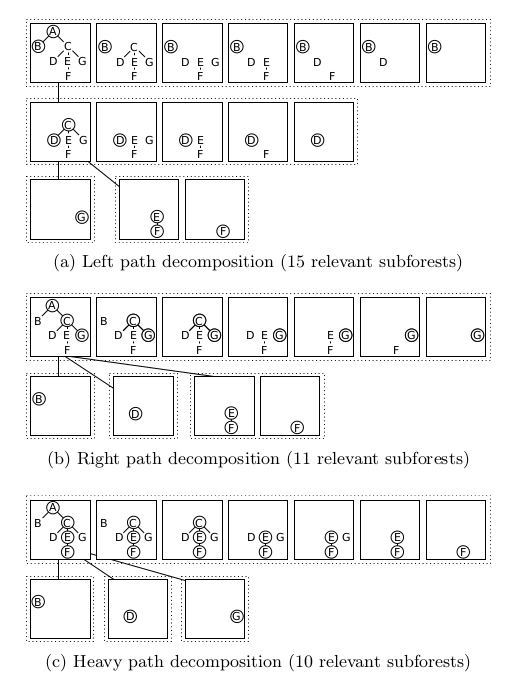
\includegraphics[width=85mm, height=100mm]{../img/LRH_decomposition.png}
\caption{Celková dekompozícia pomocou LRH strategií \citenum{RTED}}
\label{obr:LRH_decomposition}
\end{figure}

Nasledujúca lemma, ktorú pre $heavy$ cesty dokázali \citet{DMRW}
a~pre $left$ cesty zase \citet{ZHANGSHASHA}
\footnote{Pre $right$ cesty to platí obdobne, stačí nám zmeniť poradie medzi potomkami vrcholov}
nám ukáže, že počet problémov ktoré potrebujeme vyrátať závisí od výberu dekompozičnej stratégie.

\begin{lemma}
  Počet podproblémov (relevant subproblems) počítaných $SinglePath$ funkciou pre dvojicu
  stromov \tree{F} a~\tree{G} je rovná
  \begin{align*}
    \# = 
    \begin{cases}
      \abs{F} \times \abs{\FrelevantSubforests(G, \Gamma^{L}(G))} & \text{pre $left$ cesty}
      \\
      \abs{F} \times \abs{\FrelevantSubforests(G, \Gamma^{R}(G))} & \text{pre $right$ cesty}
      \\
      \abs{F} \times \abs{\AfullDecomposition(G)} & \text{pre $heavy$ cesty}
    \end{cases}
  \end{align*}
\end{lemma}

\begin{lemma}
  Minimálny počet podproblémov (cena počítania danou stratégiou),
  ktoré potrebujeme vyrátať pri použití GTEDu je
  \begin{align*}
    cena(F, G) = min
    \begin{cases}
      \abs{F} \times \abs{\AfullDecomposition(G)} &+ \rtedCostSum{F}{H}{G}
      \\
      \abs{G} \times \abs{\AfullDecomposition(F)} &+ \rtedCostSum{G}{H}{F}
      \\
      \abs{F} \times \abs{\FrelevantSubforests(G, \Gamma^{L}(G))} &+ \rtedCostSum{F}{L}{G}
      \\
      \abs{G} \times \abs{\FrelevantSubforests(F, \Gamma^{L}(F))} &+ \rtedCostSum{G}{L}{F}
      \\
      \abs{F} \times \abs{\FrelevantSubforests(G, \Gamma^{R}(G))} &+ \rtedCostSum{F}{R}{G}
      \\
      \abs{G} \times \abs{\FrelevantSubforests(F, \Gamma^{R}(F))} &+ \rtedCostSum{G}{R}{F}
    \end{cases}
  \end{align*}
  pričom $\Gamma^{L}$ a~$\Gamma^{R}$ sú funkcie vracajúce $left$ a~$right$ cestu v~lese.
\end{lemma}

\begin{dukaz}
  Je uvedený v~článku od \citet{RTED}
\end{dukaz}

Popíšeme algoritmus \ref{alg:rted} - RTED, od tvorcov \citet{RTED}.
Vďaka jeho rýchlosti \O{$n^2$} si optimálnu stratégiu nájdeme a~aj vypočítame
$GTED$ v~čase \O{$n^3$}.

\begin{algorithm}
  \caption{Optimal strategy}
  \label{alg:rted}
  \begin{algorithmic}[1]
    \Procedure {rted}{$F, G$}
      \State $L_{v}, R_{v}, H_{v} \gets$ arrays $\abs{F} \times \abs{G}$
      \State $L_{w}, R_{w}, H_{w} \gets$ arrays $\abs{G}$
      \ForAll {$v$ postorder in $F$}
        \ForAll {$w$ postorder in $G$}
          \If {$v$ is leaf}
            \State $L_{v}[v, w] \gets R_{v}[v, w] \gets H_{v}[v, w] \gets 0$
          \EndIf
          \If {$w$ is leaf}
            \State $L_{w}[w] \gets R_{w}[w] \gets  H_{w}[w] \gets 0$
          \EndIf

          \State $C := \set{$
            \Indent
              \State $(\abs{F_{v}} \times \AfullDecomposition(G_{w}) +
                H_{v}[v, w], \gamma^{H}(F)),$
              \State $(\abs{G_{w}} \times \AfullDecomposition(F_{v}) +
                H_{w}[w], \gamma^{H}(G)),$
              \State $(\abs{F_{v}} \times
                \abs{\FrelevantSubforests(G_{w}, \Gamma^{L}(G))} +
                L_{v}[v, w], \gamma^{L}(F)),$
              \State $(\abs{G_{w}} \times
                \abs{\FrelevantSubforests(F_{v}, \Gamma^{L}(F)}) +
                L_{w}[w], \gamma^{L}(G)),$
              \State $(\abs{F_{v}} \times
                \abs{\FrelevantSubforests(G_{w}, \Gamma^{R}(G))} +
                R_{v}[v, w], \gamma^{R}(F)),$
              \State $(\abs{G_{w}} \times
                \abs{\FrelevantSubforests(F_{v}, \Gamma^{R}(F))} +
                R_{w}[w], \gamma^{R}(G))$
              \State $}$
            \EndIndent

            \State Get $(c_{min}, \gamma_{min}) \in C$ such that
              $c_{min} = min \set{c' | (c', \gamma') \in C}$
            \State $Strategies[v, w] := \gamma_{min}$

            \If {$v$ is not root of tree}
            \State \Call{update}{$L_{v}$, v, w, $c_{min}$, $\gamma^{L}(parent(v)$}
              \State \Call{update}{$R_{v}$, v, w, $c_{min}$, $\gamma^{R}(parent(v)$}
              \State \Call{update}{$H_{v}$, v, w, $c_{min}$, $\gamma^{H}(parent(v)$}
            \EndIf
            \If {$w$ is not root of tree}
              \State \Call{update}{$L_{w}$, w, $c_{min}$, $\gamma^{L}(parent(w)$}
              \State \Call{update}{$R_{w}$, w, $c_{min}$, $\gamma^{R}(parent(w)$}
              \State \Call{update}{$H_{w}$, w, $c_{min}$, $\gamma^{H}(parent(w)$}
            \EndIf
        \EndFor
      \EndFor
      \State \Return {$Strategies$}
    \EndProcedure

  \item[]

    \Procedure {update}{$Table, v, w, c_{min}, \gamma$}
      \State $Table[parent(v), w] \pluseq
        \begin{cases}
          Table[v, w] & \text{if $v \in \gamma$}
          \\
          c_{min} & \text{otherwise}
        \end{cases}$
    \EndProcedure

    \Procedure {update}{$Table, w, c_{min}, \gamma$}
      \State $Table[parent(w)] \quad \pluseq
        \begin{cases}
          Table[w] & \quad \text{if $v \in \gamma$}
          \\
          c_{min} & \quad \text{otherwise}
        \end{cases}$
    \EndProcedure
  \end{algorithmic}
\end{algorithm}

Algoritmus prechádza vrcholmi stromov a~spočíta si, aká je optimálna dekompozičná stratégia
pre danú dvojicu podstromov, teda pri akej potrebujem vyrátať minimálny počet podproblémov.

Stromom prechádza v~postorder poradí, teda najprv navštívi potomkov zľava doprava, a~až tak
samotný vrchol.
Toto poradie je zvolené kvôli tomu, aby sa znížila pamäťová náročnosť a~nemuseli ukladať hodnoty
medzi všetkými dvojicami podstromov. Namiesto toho inkrementujeme hodnotu v~rodičovskom vrchole
(procedúry $Update$) pri každej návšteve jeho potomka.

\begin{lemma}
  Algoritmus \ref{alg:rted} vyráta optimalnú LRH stratégiu pre dvojicu podstromov \tree{F} a~\tree{G}
  a~časová náročnosť algoritmu je \O{$n^2$}.
\end{lemma}

\begin{dukaz}
  Je uvedený v~článku od \citet{RTED}.
\end{dukaz}

